\documentclass[12pt,a4paper]{article}

% بسته‌های مورد نیاز برای ریاضیات و فیزیک
\usepackage{amsmath}
\usepackage{amssymb}
\usepackage{amsfonts}
\usepackage{geometry}
\usepackage{color}
\usepackage[]{tcolorbox}
\usepackage{tikz} % بسته تیک‌زد برای رسم دیاگرام‌های برداری داخل متن

% تنظیمات حاشیه صفحه
\geometry{left=2cm, right=2cm, top=2.5cm, bottom=2.5cm}



% بسته زی‌پرشین برای تایپ فارسی (باید آخرین بسته باشد)
\usepackage{xepersian}
\settextfont[Scale=0.88]{Dibaj}
\setdigitfont[Scale=0.88]{Dibaj}

\title{\textbf{جزوه جامع و تحلیلی الکترومغناطیس ۲: از استخراج معادله موج تا تحلیل هندسی جواب دالامبر}}
\author{تحلیل، بسط و یکپارچه‌سازی مفاهیم کلاس}
\date{}

\begin{document}
\maketitle

\section*{مقدمه کل‌نگر}
هدف این جزوه، ارائه یک سیر منطقی و یکپارچه از مفاهیم تدریس‌شده در این جلسه کلاس الکترومغناطیس ۲ است. در این جلسه، مطالب در سه گام اساسی تکامل یافته‌اند:
\begin{enumerate}
    \item \textbf{استخراج معادله موج الکترومغناطیسی:} ابتدا با استفاده از معادلات بنیادی ماکسول، رفتار میدان‌های الکتریکی و مغناطیسی در یک محیط رسانا و اتلافی استخراج می‌شود و به معادله تلگرافچی می‌رسیم.
    \item \textbf{بررسی ریاضی جواب‌های موج تخت روان:} در گام دوم، با فرض محیط ساده‌ترِ بدون اتلاف، رفتار پتانسیل برداری $\vec{A}$ را تحلیل کرده و صدق کردن جواب‌های کلاسیک موج تخت روان $\vec{A}(\hat{k}\cdot\vec{r}-vt)$ را اثبات می‌کنیم.
    \item \textbf{حل عمومی معادله موج به روش دالامبر:} در نهایت، به جای حدس زدن شکل جواب، معادله موج را در یک بعد به کمک روش مشخصه‌ها به صورت ریاضی حل کرده و با برگرداندن آن به حالت سه‌بعدی، تعبیر هندسی زیبایی از جبهه‌های موج تخت و صفحات هم‌فاز ارائه می‌دهیم.
\end{enumerate}

\hrule
\vspace{0.5cm}

\section{معادلات بنیادی و استخراج معادله موج در محیط رسانا}
برای شروع، به بنیادی‌ترین ابزارهای الکترومغناطیس، یعنی معادلات ماکسول در فرم دیفرانسیلی (ماکروسکوپیک) نیاز داریم:

\begin{align}
	\vec{\nabla} \cdot \vec{D} &= \rho \quad &\text{(قانون گائوس)} \label{eq:gauss} \\
	\vec{\nabla} \times \vec{E} &= -\frac{\partial \vec{B}}{\partial t} \quad &\text{(قانون فارادی)} \label{eq:faraday} \\
	\vec{\nabla} \cdot \vec{B} &= 0 \quad &\text{(قانون گائوس در مغناطیس)} \label{eq:gauss_mag} \\
	\vec{\nabla} \times \vec{H} &= \vec{J} + \frac{\partial \vec{D}}{\partial t} \quad &\text{(قانون تعمیم‌یافته آمپر)} \label{eq:ampere}
\end{align}

\subsection*{روابط ساختاری و ویژگی‌های محیط}
محیطی که موج در آن منتشر می‌شود دارای ویژگی‌های خاصی است:
\begin{itemize}
	\item \textbf{روابط خطی:} $\vec{B} = \mu\vec{H}$ و $\vec{D} = \epsilon\vec{E}$. محیط همگن و ایزوتروپیک فرض شده است.
	\item \textbf{عدم وجود بار آزاد خالص ($\rho = 0$):} در یک رسانای خوب، هرگونه تجمع بار الکتریکی آزاد با سرعت بسیار بالایی (در مرتبه زمان رهاسازی $\tau = \epsilon/g$) به سطح رسانا منتقل می‌شود؛ بنابراین در داخل حجم رسانا چگالی بار حجمی صفر است.
	\item \textbf{قانون اهم دیفرانسیلی ($\vec{J} = g\vec{E}$):} حضور میدان الکتریکی متغیر با زمان، باعث ایجاد جریان الکتریکی انتقالی در رسانا می‌شود. پارامتر $g$ در اینجا همان رسانایی الکتریکی ($\sigma$) است.
\end{itemize}

با اعمال این شرایط در معادلات \eqref{eq:gauss} تا \eqref{eq:ampere}، دستگاه معادلات ماکسول برای داخل محیط رسانا به فرم ساده‌شده‌ی زیر در می‌آید:

\begin{align}
	\vec{\nabla} \cdot \vec{E} &= 0 \label{eq:sim1} \\
	\vec{\nabla} \times \vec{E} &= -\frac{\partial \vec{B}}{\partial t} \label{eq:sim2} \\
	\vec{\nabla} \cdot \vec{B} &= 0 \label{eq:sim3} \\
	\vec{\nabla} \times \vec{B} &= \mu g \vec{E} + \mu \epsilon \frac{\partial \vec{E}}{\partial t} \label{eq:sim4}
\end{align}

\subsection{استخراج معادله موج برای میدان الکتریکی}
برای رسیدن به معادله‌ای که رفتار فضایی و زمانی تنها \textbf{یک} میدان (در اینجا میدان الکتریکی $\vec{E}$) را توصیف کند، باید میدان مغناطیسی ($\vec{B}$) را از معادلات حذف کنیم.

از معادله قانون فارادی \eqref{eq:sim2} شروع کرده و از هر دو طرف آن عملگر کرل ($\vec{\nabla} \times$) می‌گیریم:
\begin{equation}
	\vec{\nabla} \times (\vec{\nabla} \times \vec{E}) = \vec{\nabla} \times \left( -\frac{\partial \vec{B}}{\partial t} \right)
\end{equation}
با توجه به اینکه عملگرهای مشتق مکانی (کرل) و مشتق زمانی مستقل هستند و می‌توانند جابه‌جا شوند، سمت راست را بازنویسی می‌کنیم:
\begin{equation} \label{eq:curl_curl}
	\vec{\nabla} \times \vec{\nabla} \times \vec{E} = -\frac{\partial}{\partial t} (\vec{\nabla} \times \vec{B})
\end{equation}

\subsubsection*{ساده‌سازی سمت چپ (اتحاد برداری)}
اتحاد برداری معروف «کرلِ کرل» به صورت زیر است:
\begin{equation*}
	\vec{\nabla} \times \vec{\nabla} \times \vec{E} = \vec{\nabla}(\vec{\nabla} \cdot \vec{E}) - \nabla^2\vec{E}
\end{equation*}
طبق معادله \eqref{eq:sim1}، دیورژانس میدان الکتریکی صفر است ($\vec{\nabla} \cdot \vec{E} = 0$). پس جمله اول حذف شده و سمت چپ تنها برابر با $-\nabla^2\vec{E}$ خواهد بود.

\subsubsection*{ساده‌سازی سمت راست (جایگذاری قانون آمپر)}
اکنون معادله \eqref{eq:sim4} را در سمت راست معادله \eqref{eq:curl_curl} جایگذاری می‌کنیم:
\begin{equation*}
	-\frac{\partial}{\partial t} (\vec{\nabla} \times \vec{B}) = -\frac{\partial}{\partial t} \left( \mu g \vec{E} + \mu \epsilon \frac{\partial \vec{E}}{\partial t} \right) = -\mu g \frac{\partial \vec{E}}{\partial t} - \mu \epsilon \frac{\partial^2 \vec{E}}{\partial t^2}
\end{equation*}

با برابر قرار دادن سمت چپ و راست، علامت‌های منفی از طرفین ساده می‌شوند و به \textbf{معادله موج در محیط رسانا (معادله تلگرافچی)} می‌رسیم:

\begin{tcolorbox}[colback=blue!5,colframe=blue!50!black,title=معادله دیفرانسیل موج الکترومغناطیسی]
\begin{equation} \label{eq:telegraph}
	\nabla^2 \vec{E} = \mu g \frac{\partial \vec{E}}{\partial t} + \mu \epsilon \frac{\partial^2 \vec{E}}{\partial t^2}
\end{equation}
\end{tcolorbox}

\subsubsection*{شهود فیزیکی جملات:}
\begin{itemize}
	\item \textbf{جمله $\mu \epsilon \frac{\partial^2 \vec{E}}{\partial t^2}$ (جمله انتشار):} این مشتق مرتبه دوم زمانی، عامل اصلی ایجاد رفتار موجی و انتشار انرژی در فضاست (مانند نوسانگر هماهنگ).
	\item \textbf{جمله $\mu g \frac{\partial \vec{E}}{\partial t}$ (جمله میرایی/اتلاف):} حضور مشتق مرتبه اول زمانی به معنای اتلاف انرژی است. از نظر فیزیکی، میدان الکتریکی موج باعث ایجاد جریان $g\vec{E}$ در رسانا شده و طبق قانون ژول، انرژی الکترومغناطیسی به صورت گرما تلف می‌شود. این جمله باعث افت نمایی دامنه موج در حین نفوذ به رسانا می‌شود (پدیده اثر پوستی یا \lr{Skin Effect}).
\end{itemize}

\subsection{سرعت موج، ضریب شکست و عملگر دالامبر}
\subsubsection*{سرعت موج و ضریب شکست}
اگر محیط رسانا نبود ($g=0$)، معادله به فرم استاندارد موج $\nabla^2 \vec{E} = \frac{1}{v^2}\frac{\partial^2 \vec{E}}{\partial t^2}$ در می‌آمد. سرعت فاز موج در محیط برابر است با:
\begin{equation}
	v = \frac{1}{\sqrt{\mu\epsilon}} = \frac{1}{\sqrt{\mu_0 \epsilon_0} \sqrt{\mu_r \epsilon_r}}
\end{equation}
با توجه به اینکه سرعت نور در خلأ $c = \frac{1}{\sqrt{\mu_0 \epsilon_0}}$ است، و با تعریف ثابت‌های نسبی به فرم $K_m = \mu_r$ و $K = \epsilon_r$، داریم:
\begin{equation}
	v = \frac{c}{\sqrt{K_m K}}
\end{equation}
برای اکثر دی‌الکتریک‌ها و محیط‌های کاربردی غیرمغناطیسی، نفوذپذیری مغناطیسی نسبی تقریباً یک است ($K_m \approx 1$). در این صورت $\sqrt{K} = n$ تعریف می‌شود که همان \textbf{ضریب شکست \lr{(Refractive Index)}} محیط است.

\subsubsection*{فرم فشرده با عملگر دالامبر \lr{(d'Alembertian)}}
در فیزیک نظری و نسبیت، برای نمایش فشرده‌تر معادلات موج از عملگر دالامبر $(\Box^2)$ استفاده می‌شود که یک لاپلاسین چهاربعدی (مکان-زمان) است:
\begin{equation}
	\Box^2 \equiv \nabla^2 - \frac{1}{v^2}\frac{\partial^2}{\partial t^2} = \nabla^2 - \mu\epsilon\frac{\partial^2}{\partial t^2}
\end{equation}

اگر همه جملات معادله موج را به یک سمت ببریم:
\begin{equation*}
	\left( \nabla^2 - \mu \epsilon \frac{\partial^2}{\partial t^2} \right) \vec{E} = \mu g \frac{\partial \vec{E}}{\partial t}
\end{equation*}

که با استفاده از عملگر دالامبر به فرم زیر نوشته می‌شود:
\begin{align}
	\Box^2 \vec{E} &= \mu g \frac{\partial \vec{E}}{\partial t} \label{eq:boxE} \\
	\Box^2 \vec{B} &= \mu g \frac{\partial \vec{B}}{\partial t} \label{eq:boxB}
\end{align}
(اثبات برای میدان مغناطیسی $\vec{B}$ نیز کاملاً مشابه است، با این تفاوت که ابتدا از قانون آمپر کرل می‌گیریم).

\vspace{0.5cm}
\begin{tcolorbox}[colback=gray!8, colframe=gray!75, title=\textbf{گذار مفهومی ۱: عبور از اتلاف و گذار به پتانسیل برداری}]
پس از بررسی معادله موج الکترومغناطیسی در محیط‌های رسانا و مشاهده چگونگی ایجاد رفتار میرونده به دلیل حضور جمله اتلافی $\mu g \frac{\partial \vec{E}}{\partial t}$، اکنون گام بعدی در تحلیل رفتار امواج، بررسی جواب‌های ریاضی این معادلات است.

برای ساده‌سازی تحلیل ریاضی و فهم فیزیکی پایه‌ای، میدان‌ها را در یک محیط ساده، همگن و کاملاً نارسانا (بدون اتلاف، $g=0$ و در فضای بدون بار آزاد، $\rho=0$) بررسی می‌کنیم. همچنین، به جای تحلیل مستقیم میدان‌های برداری هم‌بسته $\vec{E}$ و $\vec{B}$، ترجیح می‌دهیم معادله موج را بر حسب پتانسیل برداری مغناطیسی $\vec{A}$ در گیج لورنتز فرمول‌بندی کنیم. این رویکرد به ما اجازه می‌دهد که ویژگی‌های ذاتی انتشار موج را به شیوه‌ای یکپارچه مطالعه کنیم.
\end{tcolorbox}
\vspace{0.5cm}

\section{اثبات جواب موج تخت برای پتانسیل برداری}
تحت شرایط بدون اتلاف و بدون منبع ذکر شده در گذار فوق، پتانسیل برداری $\vec{A}$ (که میدان‌های فیزیکی $\vec{E}$ و $\vec{B}$ از روی آن طبق روابط میدان-پتانسیل استخراج می‌شوند) در گیج لورنتز در معادله دیفرانسیل موج همگن صدق می‌کند:
\begin{equation} \label{eq:wave_pot}
    \left( \nabla^2 - \frac{1}{v^2} \frac{\partial^2}{\partial t^2} \right) \vec{A} = 0
\end{equation}
که در آن $v = 1/\sqrt{\mu\epsilon}$ سرعت انتشار موج در این محیط است.

\subsection{تعریف متغیر فاز و جواب پیشنهادی موج تخت}
قصد داریم ثابت کنیم که تابعی به فرم یک موج تخت روان \lr{(Traveling Plane Wave)}، جواب دقیق و معتبر معادله موج بالا است.

برای این کار، یک متغیر اسکالر به نام «فاز» با نماد $\xi$ تعریف می‌کنیم:
\begin{equation}
    \xi = \hat{k} \cdot \vec{r} - vt
\end{equation}
اگر بردار مکان $\vec{r} = x\hat{i} + y\hat{j} + z\hat{k}$ و بردار یکه جهت انتشار موج $\hat{k} = k_x\hat{i} + k_y\hat{j} + k_z\hat{k}$ باشد، ضرب داخلی آن‌ها فاز را به شکل مختصاتی زیر درمی‌آورد:
\begin{equation}
    \xi = k_x x + k_y y + k_z z - vt
\end{equation}

\begin{tcolorbox}[colback=yellow!5,colframe=red!50!black,title=نکته بسیار مهم فیزیکی (تله ریاضی)]
توجه داشته باشید که در اینجا بردار $\hat{k}$ یک \textbf{بردار یکه \lr{(Unit Vector)}} در راستای انتشار موج است، نه بردار عدد موج ($\vec{k}$). بنابراین، مؤلفه‌های $k_x, k_y, k_z$ در واقع کسینوس‌های هادی جهت انتشار هستند و باید همیشه شرط زیر برای آن‌ها برقرار باشد:
\begin{equation} \label{eq:unit_vec}
    |\hat{k}|^2 = k_x^2 + k_y^2 + k_z^2 = 1
\end{equation}
\end{tcolorbox}

فرض می‌کنیم پتانسیل برداری تنها تابعی از این متغیر فاز باشد، یعنی $\vec{A} = \vec{A}(\xi)$. اکنون باید نشان دهیم که این تابع در معادله موج \eqref{eq:wave_pot} صدق می‌کند.

\subsection{اعمال عملگر لاپلاسین (محاسبه مشتقات مکانی)}
برای محاسبه $\nabla^2 \vec{A}$، باید مشتقات جزئی مرتبه دوم $\vec{A}$ را نسبت به متغیرهای مکانی $x, y, z$ محاسبه کنیم. چون $\vec{A}$ تابعی از $\xi$ و خود $\xi$ تابعی از مختصات است، استفاده از قاعده زنجیره‌ای \lr{(Chain Rule)} الزامی است.

\subsubsection*{محاسبه مشتقات در راستای محور $x$}
مشتق اول نسبت به $x$:
\begin{equation}
    \frac{\partial \vec{A}}{\partial x} = \frac{\partial \vec{A}}{\partial \xi} \frac{\partial \xi}{\partial x}
\end{equation}
از تعریف فاز می‌دانیم که $\frac{\partial \xi}{\partial x} = k_x$. پس:
\begin{equation}
    \frac{\partial \vec{A}}{\partial x} = k_x \frac{\partial \vec{A}}{\partial \xi}
\end{equation}

برای یافتن مشتق دوم، دوباره عملگر $\frac{\partial}{\partial x}$ را روی نتیجه اعمال می‌کنیم. مجدداً با استفاده از قاعده زنجیره‌ای، به این معنی که $\frac{\partial}{\partial x} \equiv \frac{\partial \xi}{\partial x} \frac{\partial}{\partial \xi}$، داریم:
\begin{equation}
    \frac{\partial^2 \vec{A}}{\partial x^2} = \frac{\partial}{\partial x} \left( k_x \frac{\partial \vec{A}}{\partial \xi} \right) = \frac{\partial}{\partial \xi} \left( k_x \frac{\partial \vec{A}}{\partial \xi} \right) \cdot \frac{\partial \xi}{\partial x}
\end{equation}
\begin{equation}
    \frac{\partial^2 \vec{A}}{\partial x^2} = \left( k_x \frac{\partial^2 \vec{A}}{\partial \xi^2} \right) \cdot (k_x) = k_x^2 \frac{\partial^2 \vec{A}}{\partial \xi^2}
\end{equation}

\subsubsection*{تعمیم به سایر مؤلفه‌ها و تشکیل لاپلاسین}
به دلیل تقارن کامل ریاضی، مشتقات دوم نسبت به $y$ و $z$ نیز نتایج کاملاً مشابهی خواهند داشت:
\begin{equation}
    \frac{\partial^2 \vec{A}}{\partial y^2} = k_y^2 \frac{\partial^2 \vec{A}}{\partial \xi^2} \quad , \quad \frac{\partial^2 \vec{A}}{\partial z^2} = k_z^2 \frac{\partial^2 \vec{A}}{\partial \xi^2}
\end{equation}

عملگر لاپلاسین برابر است با مجموع این سه مشتق دوم مکانی ($\nabla^2 = \frac{\partial^2}{\partial x^2} + \frac{\partial^2}{\partial y^2} + \frac{\partial^2}{\partial z^2}$). با جمع کردن روابط بالا داریم:
\begin{equation}
    \nabla^2 \vec{A} = (k_x^2 + k_y^2 + k_z^2) \frac{\partial^2 \vec{A}}{\partial \xi^2}
\end{equation}
با جایگذاری شرط بردار یکه از رابطه \eqref{eq:unit_vec} که مقدار پرانتز را برابر ۱ می‌کند، نتیجه به دست می‌آید:
\begin{equation} \label{eq:laplacian_result}
    \nabla^2 \vec{A} = (1) \frac{\partial^2 \vec{A}}{\partial \xi^2} = \frac{\partial^2 \vec{A}}{\partial \xi^2}
\end{equation}

\subsection{محاسبه مشتقات زمانی}
اکنون باید بخش دوم معادله موج، یعنی مشتقات نسبت به زمان $t$ را بیابیم. دوباره از قاعده زنجیره‌ای استفاده می‌کنیم:
\begin{equation}
    \frac{\partial \vec{A}}{\partial t} = \frac{\partial \vec{A}}{\partial \xi} \frac{\partial \xi}{\partial t}
\end{equation}
از تعریف فاز، مشتق آن نسبت به زمان برابر $\frac{\partial \xi}{\partial t} = -v$ است. پس:
\begin{equation}
    \frac{\partial \vec{A}}{\partial t} = -v \frac{\partial \vec{A}}{\partial \xi}
\end{equation}
با اعمال مشتق دوم نسبت به زمان:
\begin{equation}
    \frac{\partial^2 \vec{A}}{\partial t^2} = \frac{\partial}{\partial t} \left( -v \frac{\partial \vec{A}}{\partial \xi} \right) = \frac{\partial}{\partial \xi} \left( -v \frac{\partial \vec{A}}{\partial \xi} \right) \cdot \frac{\partial \xi}{\partial t}
\end{equation}
\begin{equation} \label{eq:time_result}
    \frac{\partial^2 \vec{A}}{\partial t^2} = \left( -v \frac{\partial^2 \vec{A}}{\partial \xi^2} \right) \cdot (-v) = v^2 \frac{\partial^2 \vec{A}}{\partial \xi^2}
\end{equation}

\subsection{اثبات نهایی صدق در معادله موج}
در مرحله آخر، نتایج به دست آمده برای لاپلاسین (رابطه \eqref{eq:laplacian_result}) و مشتق دوم زمانی (رابطه \eqref{eq:time_result}) را در معادله اصلی موج \eqref{eq:wave_pot} قرار می‌دهیم:
\begin{equation}
    \nabla^2 \vec{A} - \frac{1}{v^2}\frac{\partial^2 \vec{A}}{\partial t^2} = 0
\end{equation}
\begin{equation}
    \frac{\partial^2 \vec{A}}{\partial \xi^2} - \frac{1}{v^2} \left( v^2 \frac{\partial^2 \vec{A}}{\partial \xi^2} \right) = 0
\end{equation}
با ساده شدن $v^2$ در صورت و مخرج جمله دوم داریم:
\begin{equation}
    \frac{\partial^2 \vec{A}}{\partial \xi^2} - \frac{\partial^2 \vec{A}}{\partial \xi^2} = 0 \quad \implies \quad 0 = 0
\end{equation}

این تساوی قطعی اثبات می‌کند که هر تابع دلخواهی به فرم $\vec{A}(\hat{k}\cdot\vec{r} - vt)$ پاسخی ریاضی و معتبر برای معادله موج است. این پاسخ‌ها معرف جبهه موج تخت با فاز ثابت هستند که با سرعت $v$ در جهت $\hat{k}$ حرکت می‌کنند.

\vspace{0.5cm}
\begin{tcolorbox}[colback=gray!8, colframe=gray!75, title=\textbf{گذار مفهومی ۲: از راستی‌آزمایی جواب تا استخراج جواب عمومی دالامبر}]
تا بدین‌جا، ما یک فرم خاص از جواب را پیشنهاد داده (موج تخت با فاز $\hat{k}\cdot\vec{r} - vt$) و صحت آن را در معادله موج به صورت ریاضی بررسی و تایید کردیم. اما این رویکرد متکی بر داشتن یک «حدس اولیه» بود. سوالی که به عنوان یک فیزیکدان باید از خود بپرسیم این است: عمومی‌ترین و کلی‌ترین جواب ریاضی برای یک معادله موج چیست؟ آیا می‌توان بدون هیچ حدس قبلی، مستقیماً از روی خود معادله دیفرانسیل به این جواب‌ها رسید؟

پاسخ مثبت است. برای پاسخ به این سوال و پرهیز از پیچیدگی‌های چندبعدی هندسی، مسئله را به یک بعد تقلیل می‌دهیم. با محدود کردن فضا به راستای محور $x$، از روش تاریخی ژان دالامبر استفاده می‌کنیم. در این روش، با تعریف متغیرهای مشخصه، معادله دیفرانسیل با مشتقات جزئی را حل کرده و نشان خواهیم داد که چگونه مفهوم فیزیکی موج پیشرونده و پس‌رونده به طور طبیعی از بطن ریاضیات خارج می‌شود. سپس بار دیگر به فضای سه‌بعدی بازگشته و تعبیر هندسی کامل‌تری از صفحات هم‌فاز ارائه می‌دهیم.
\end{tcolorbox}
\vspace{0.5cm}

\section{حل دالامبر برای معادله موج و تعبیر هندسی موج تخت}
کار را با معادله موج یک‌بعدی برای تابع اسکالر $u(x,t)$ آغاز می‌کنیم:
\begin{equation} \label{eq:wave1d}
    \frac{\partial^2 u}{\partial x^2} - \frac{1}{v^2} \frac{\partial^2 u}{\partial t^2} = 0
\end{equation}

\subsection{تغییر متغیر متقارن و انتقال به مختصات مشخصه}
برای ایجاد تقارن بین بخش مکانی ($x$) و زمانی ($t$) در معادله، تغییر متغیر ساده‌ی $y = vt$ را اعمال می‌کنیم. با این کار مشتق زمانی به شکل زیر تبدیل می‌شود:
\begin{equation}
    \frac{\partial u}{\partial t} = \frac{\partial u}{\partial y}\frac{\partial y}{\partial t} = v \frac{\partial u}{\partial y} \implies \frac{\partial^2 u}{\partial t^2} = v^2 \frac{\partial^2 u}{\partial y^2}
\end{equation}
با جایگذاری این نتیجه در معادله \eqref{eq:wave1d}، فرم متقارن زیر حاصل می‌شود:
\begin{equation} \label{eq:sym_wave}
    \frac{\partial^2 u}{\partial x^2} - \frac{\partial^2 u}{\partial y^2} = 0
\end{equation}

برای حل معادله \eqref{eq:sym_wave}، از تکنیک تغییر متغیر به «مختصات مشخصه» \lr{(Characteristic Coordinates)} استفاده می‌کنیم. متغیرهای جدید $x'$ و $y'$ را به صورت زیر تعریف می‌کنیم:
\begin{align}
    x' &= x + y \label{eq:xp} \\
    y' &= x - y \label{eq:yp}
\end{align}
اکنون باید عملگرهای مشتق‌گیری $\frac{\partial}{\partial x}$ و $\frac{\partial}{\partial y}$ را بر حسب متغیرهای جدید بازنویسی کنیم.

\subsubsection*{اعمال قاعده زنجیره‌ای}
برای مشتق‌گیری از تابع $u$ نسبت به $x$ داریم:
\begin{equation}
    \frac{\partial u}{\partial x} = \frac{\partial u}{\partial x'}\frac{\partial x'}{\partial x} + \frac{\partial u}{\partial y'}\frac{\partial y'}{\partial x}
\end{equation}
با توجه به روابط \eqref{eq:xp} و \eqref{eq:yp}، می‌دانیم که $\frac{\partial x'}{\partial x} = 1$ و $\frac{\partial y'}{\partial x} = 1$. پس:
\begin{equation} \label{eq:du_dx}
    \frac{\partial u}{\partial x} = \frac{\partial u}{\partial x'} + \frac{\partial u}{\partial y'} \quad \implies \quad \frac{\partial}{\partial x} \equiv \frac{\partial}{\partial x'} + \frac{\partial}{\partial y'}
\end{equation}
به طریق مشابه برای مشتق نسبت به $y$ (با توجه به اینکه $\frac{\partial x'}{\partial y} = 1$ و $\frac{\partial y'}{\partial y} = -1$):
\begin{equation} \label{eq:du_dy}
    \frac{\partial u}{\partial y} = \frac{\partial u}{\partial x'} - \frac{\partial u}{\partial y'} \quad \implies \quad \frac{\partial}{\partial y} \equiv \frac{\partial}{\partial x'} - \frac{\partial}{\partial y'}
\end{equation}

\subsubsection*{محاسبه مشتقات مرتبه دوم}
اکنون مشتقات دوم مورد نیاز در معادله \eqref{eq:sym_wave} را تشکیل می‌دهیم:
\begin{equation}
    \frac{\partial^2 u}{\partial x^2} = \left( \frac{\partial}{\partial x'} + \frac{\partial}{\partial y'} \right) \left( \frac{\partial u}{\partial x'} + \frac{\partial u}{\partial y'} \right) = \frac{\partial^2 u}{\partial x'^2} + 2\frac{\partial^2 u}{\partial x'\partial y'} + \frac{\partial^2 u}{\partial y'^2}
\end{equation}
\begin{equation}
    \frac{\partial^2 u}{\partial y^2} = \left( \frac{\partial}{\partial x'} - \frac{\partial}{\partial y'} \right) \left( \frac{\partial u}{\partial x'} - \frac{\partial u}{\partial y'} \right) = \frac{\partial^2 u}{\partial x'^2} - 2\frac{\partial^2 u}{\partial x'\partial y'} + \frac{\partial^2 u}{\partial y'^2}
\end{equation}

با کم کردن این دو رابطه از یکدیگر (طبق فرم متقارن معادله موج)، جملات اول و سوم ساده شده و تنها جمله مشتق مختلط باقی می‌ماند:
\begin{equation}
    \frac{\partial^2 u}{\partial x^2} - \frac{\partial^2 u}{\partial y^2} = 4 \frac{\partial^2 u}{\partial x' \partial y'} = 0
\end{equation}

\subsection{انتگرال‌گیری و رسیدن به جواب عمومی دالامبر}
معادله دیفرانسیل ما اکنون به فرم بسیار ساده زیر درآمده است:
\begin{equation}
    \frac{\partial}{\partial y'} \left( \frac{\partial u}{\partial x'} \right) = 0
\end{equation}
این معادله نشان می‌دهد که مشتقِ عبارت داخل پرانتز نسبت به $y'$ صفر است. بنابراین، عبارت داخل پرانتز تنها می‌تواند تابعی از متغیر دیگر یعنی $x'$ باشد:
\begin{equation}
    \frac{\partial u}{\partial x'} = \varphi(x')
\end{equation}
اکنون از طرفین نسبت به $x'$ انتگرال می‌گیریم تا خود تابع $u$ به دست آید:
\begin{equation}
    u(x', y') = \int \varphi(x') dx' + f(y')
\end{equation}
حاصل انتگرال اول را یک تابع دلخواه مانند $g(x')$ می‌نامیم و ثابت انتگرال‌گیری نیز می‌تواند تابعی دلخواه از متغیر دیگر یعنی $f(y')$ باشد:
\begin{equation}
    u(x', y') = g(x') + f(y')
\end{equation}
با برگرداندن متغیرها به حالت اولیه ($x' = x+vt$ و $y' = x-vt$)، به \textbf{جواب مشهور دالامبر \lr{(D'Alembert's Formula)}} می‌رسیم:
\begin{tcolorbox}[colback=green!5,colframe=green!50!black,title=جواب عمومی معادله موج یک‌بعدی]
\begin{equation} \label{eq:dalembert_sol}
    u(x,t) = f(x - vt) + g(x + vt)
\end{equation}
\end{tcolorbox}
\textbf{شهود فیزیکی:} تابع $f(x-vt)$ نشان‌دهنده موجی است که با سرعت $v$ در جهت مثبت محور $x$ در حال حرکت (پیشروی) است، و تابع $g(x+vt)$ موجی را نشان می‌دهد که در جهت منفی محور $x$ در حال حرکت است. این نتیجه نشان می‌دهد که هر موج یک‌بعدی، ترکیبی خطی از دو موج روان در دو جهت مخالف است.

\subsection{تعبیر هندسی و دیاگرام امواج تخت \lr{(Plane Waves)}}
در فیزیک امواج سه‌بعدی، جواب موج به فرم عمومی $u(\vec{r}, t) = f(\hat{k} \cdot \vec{r} - vt)$ تعمیم می‌یابد. در این رابطه:
\begin{itemize}
    \item $\hat{k}$ بردار یکه عمود بر جبهه موج است که جهت انتشار انرژی را نشان می‌دهد.
    \item عبارت $\xi = \hat{k} \cdot \vec{r} - vt$ متغیر فاز موج است.
\end{itemize}

دیاگرام هندسی زیر مفهوم صفحات فاز ثابت و انتشار آن‌ها را در فضا به تصویر می‌کشد:

\begin{figure}[h!]
\centering
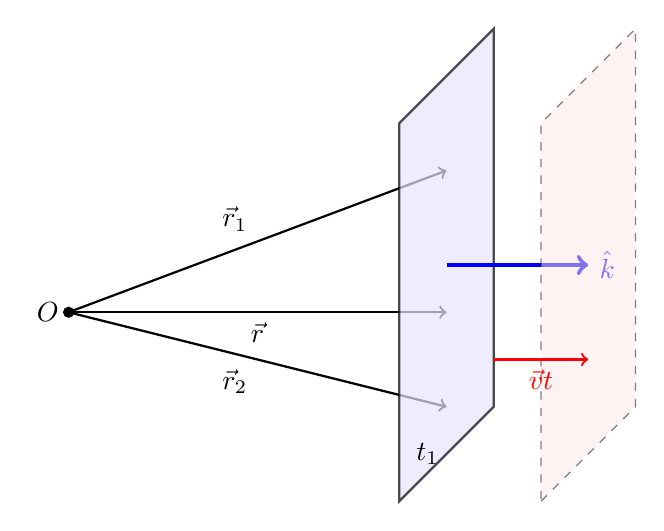
\begin{tikzpicture}[scale=1.2]
    % Origin
    \filldraw[black] (0,0) circle (1.5pt) node[left] {$O$};
    
    % Vectors to Plane 1
    \draw[thick, ->] (0,0) -- (4,1.5) node[midway, above left] {$\vec{r}_1$};
    \draw[thick, ->] (0,0) -- (4,0) node[midway, below] {$\vec{r}$};
    \draw[thick, ->] (0,0) -- (4,-1) node[midway, below left] {$\vec{r}_2$};
    
    % Plane 1 (at t1)
    \draw[thick, fill=blue!10, opacity=0.7] (3.5, -2) -- (4.5, -1) -- (4.5, 3) -- (3.5, 2) -- cycle;
    \node at (3.8, -1.5) {$t_1$};
    
    % Normal Vector k
    \draw[ultra thick, ->, blue] (4, 0.5) -- (5.5, 0.5) node[right] {$\hat{k}$};
    
    % Plane 2 (at later time, showing movement)
    \draw[dashed, fill=red!10, opacity=0.5] (5, -2) -- (6, -1) -- (6, 3) -- (5, 2) -- cycle;
    \draw[->, thick, red] (4.5, -0.5) -- (5.5, -0.5) node[midway, below] {$\vec{v}t$};
    
\end{tikzpicture}
\caption{نمایش هندسی جبهه موج تخت. تمام بردارهای مکان $\vec{r}$ که روی یک صفحه قرار دارند، تصویر یکسانی روی بردار انتشار $\hat{k}$ می‌سازند.}
\label{fig:plane_wave}
\end{figure}

\subsubsection*{تحلیل دیاگرام و تطابق با حالت یک‌بعدی:}
مطابق دیاگرام بالا، اگر مجموعه‌ای از نقاط (با بردارهای مکان $\vec{r}_1, \vec{r}, \vec{r}_2$) روی یک صفحه عمود بر $\hat{k}$ قرار داشته باشند، ضرب داخلی تمام آن‌ها با بردار $\hat{k}$ یک مقدار ثابت خواهد بود ($\hat{k} \cdot \vec{r} = \text{Constant}$). این یعنی در یک زمان مشخص $t_1$، فاز موج ($\xi$) در تمام نقاط این صفحه برابر است. به این صفحات، \textbf{صفحات هم‌فاز \lr{(Equiphase Surfaces)}} می‌گویند.

در نهایت، اگر جهت انتشار موج تنها در راستای محور $x$ باشد (یعنی جبهه موج موازی با صفحه $yz$ و بردار انتشار $\hat{k} = \hat{i}$)، ضرب داخلی به مؤلفه $x$ ساده می‌شود و فاز برابر خواهد بود با:
\begin{equation}
    \xi = x - vt
\end{equation}
این نتیجه، تطابق کامل و شگفت‌انگیز تعبیر هندسی سه‌بعدی را با آرگومان به دست آمده از حل ریاضی دالامبر یک‌بعدی یعنی $f(x-vt)$ نشان می‌دهد. بدین ترتیب درس با پیوند ریاضیات دالامبر و هندسه انتشار به کمال خود می‌رسد.

\end{document}
